After the summary step in Subsection~\ref{Summary}, aspects/features from user reviews of "Man Man" application are discovered and assigned with sentiment scores shown in Table~\ref{table:topicManMan}. 

Figure~\ref{fig:graphmanman} helps visualize and interpret the results in a bar graph format. The sentiment scores for each topic are between [-1,1] where negative number means negative sentiment and vice versa. The higher the number means higher degree of negativity or positivity. Please note that in SentiWordNet the highest positive and lowest negative sentiment scores are 0.75 and -0.75, respectively. Therefore, the sentiment score of 0.5153 can be considered very positive and -0.5156 can be considered very negative. 

\begin{table}
	\caption{20 topics/aspects/features discovered from Man Man user reviews}
	\label{table:topicManMan}
	\centering
	\begin{tabular}{|l|r|
			r|r|
		}
		\hline
		\multicolumn{1}{|c|}{topic} 
		& \multicolumn{1}{|c|}{sentiment} 
		& \multicolumn{1}{|c|}{no. of positive} 
		& \multicolumn{1}{|c|}{no. of negative}
		\\
		\hline
		{\selectlanguage{thai}เปลี่ยน ภาษา} & 0.2770 
		& 35 & 9 
		\\
		\hline
		{\selectlanguage{thai}พัฒนา ยอด} & 0.2666 
		& 47 & 6 
		\\
		\hline
		sticker {\selectlanguage{thai}หน่อย ขยาย} & 0.2046 
		& 36 & 15 
		\\
		\hline
		{\selectlanguage{thai}สะดวก สวย} & 0.3926 
		& 84 & 13 
		\\
		\hline
		{\selectlanguage{thai}สายตา ขนาด ใหญ่} & 0.5153 
		& 143 & 26 
		\\
		\hline
		{\selectlanguage{thai}ยกเว้น ทำนาย} & 0.2315 
		& 19 & 2 
		\\
		\hline
		{\selectlanguage{thai}ปรับปรุง ยาก} & 0.2035
		 & 17 & 11 
		 \\
		\hline
		{\selectlanguage{thai}ปุ่ม หาย} & -0.5156 
		& 49 & 23 
		\\
		\hline
		{\selectlanguage{thai}ชอบ แม่น} & 0.3926 
		& 142 & 14 
		\\
		\hline
		{\selectlanguage{thai}สุดยอด ลอง} & 0.3926 
		& 145 & 12 
		\\
		\hline
		{\selectlanguage{thai}แป้น รวน} & -0.3352 
		& 24 & 9 
		\\
		\hline
		{\selectlanguage{thai}แก้ไข สี} & 0.2167 
		& 40 & 15 
		\\
		\hline
		{\selectlanguage{thai}พิมพ์ ง่าย} & 0.5153 
		& 201 & 12 
		\\
		\hline
		{\selectlanguage{thai}เสียง เสียดาย} & 0.4066
		 & 17 & 4 
		 \\
		\hline
		{\selectlanguage{thai}ปรับ ขนาด ค้าง} & 0.5153 
		& 63 & 13 
		\\
		\hline
		{\selectlanguage{thai}ปุ่ม แจ่ม ซับซ้อน} & -0.5156 
		& 30 & 17 
		\\
		\hline
		{\selectlanguage{thai}เพิ่ม อิโมจิ} & 0.4066 
		& 35 & 1 
		\\
		\hline
		{\selectlanguage{thai}เดา คำ} & -0.5156 
		& 44 & 9 
		\\
		\hline
		{\selectlanguage{thai}พิมพ์ พลาด} & 0.5153 
		& 68 & 11 
		\\
		\hline
		{\selectlanguage{thai}แป้น ใหญ่} & 0.3396 
		& 82 & 13 
		\\
		\hline
	\end{tabular}
\end{table}

\begin{figure}
	\centering
	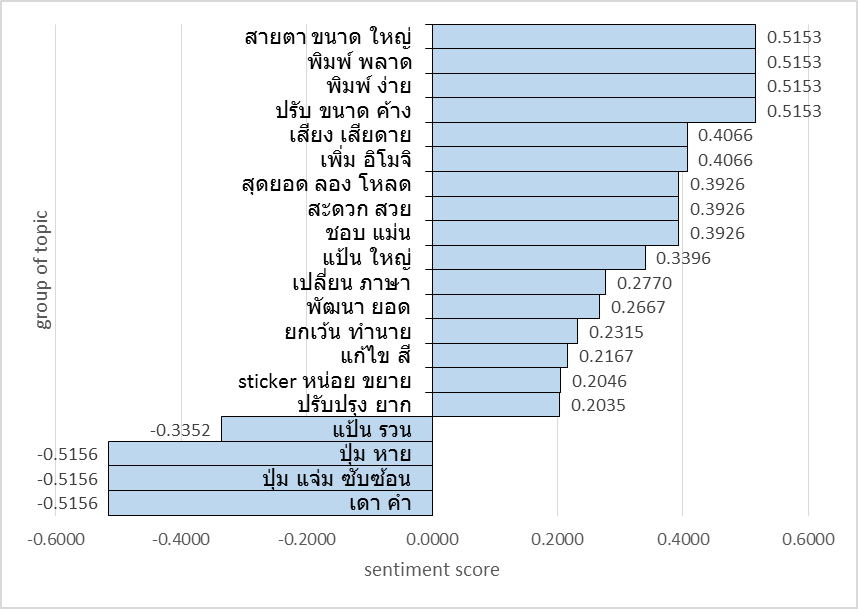
\includegraphics[width=0.9\linewidth]{graphmanman}
	\caption{sentiment score of topic from man man user reviews}
	\label{fig:graphmanman}
\end{figure}

We evaluated our approach by asking one person not related our research to manually label sentiments for each sentence whether it is positive, negative, or neutral. This information is used as truth values to calculate precision, recall, and accuracy. Table~\ref{table:f-measureSenti} shows evaluation results.

\begin{table}[h]
	\caption{F-Measure and Accuracy for Sentiment Analysis}
	\label{table:f-measureSenti}
	\centering
	\begin{tabular}{|l|r|r|r|r|}
		\hline
		\multicolumn{1}{|c|}{\textbf{Application}} &
		\multicolumn{1}{|c|}{\textbf{Precision}} &
		\multicolumn{1}{|c|}{\textbf{Recall}} &
		\multicolumn{1}{|c|}{\textbf{F-Measure}} &
		\multicolumn{1}{|c|}{\textbf{Accuracy}} \\
		\hline
		Man Man & 0.5028 & 0.3189 & 0.3570 & 0.6110\\
		\hline
		H-TV & 0.5208 & 0.2889 & 0.3366 & 0.4837 \\
		\hline
		K-Mobile & 0.4535 & 0.2810 & 0.3240 & 0.5153 \\
		\hline
	\end{tabular}
\end{table}

We did not evaluate whether the LDA produced accurate topics/aspects/features. As with most unsupervised learning technique, accuracy evaluation is difficult and also subjective. Different persons may have very different points of view on how to identify topics/aspects in large amount of data. Gunzmam and Laalej's paper~\cite{userslikefeature} also mentioned difficulties in evaluating results from topic modelling technique. Since the LDA technique is widely known and used for topic modelling, we therefore make an assumption that results from LDA is accurate at some level. 

However, when given aspect/topic/features, we are able to evaluate their sentiments. Table~\ref{table:f-measureTopic} shows the result of the evaluation whether or not the sentiment for each aspect/topic/feature is accurate. The same person that help label sentiments for sentences also help label sentiments for aspect/topic/feature. Remark that the person only lables the orientation of the sentiment whether it is positive, negative, or neutral, but did not label sentiment intensity or scores since it is much harder to evaluate and it is very subjective, even more subjective than sentiment orientations.

\begin{table}
	\caption{Precision, Recall, F-Measure and Accuracy for sentiment of topic}
	\label{table:f-measureTopic}
	\centering
	\begin{tabular}{|l|r|r|r|r|}
		\hline
		\multicolumn{1}{|c|}{\multirow{2}{*}{application}} & 
		\multicolumn{4}{|c|}{Topic} \\
		\cline{2-5}
		\multicolumn{1}{|c|}{} &
		\multicolumn{1}{|c|}{precision}&
		\multicolumn{1}{|c|}{recall}&
		\multicolumn{1}{|c|}{f-measure} &
		\multicolumn{1}{|c|}{accuracy} \\
		\hline
		Man Man & 0.7188 & 0.6538 & 0.6848 & 0.55\\
		\hline
		H-Tv & 0.5252 & 0.5333 & 0.5293 & 0.5\\
		\hline
		K-mobile & 0.2368 & 0.45 & 0.3103 & 0.45\\
		\hline
	\end{tabular}
\end{table}

\subsection*{Limitation and Possible Future Works}
Our work still has some limitations. Some are mentioned in Section~\ref{Approach} such as limitations in sentence and word segmentations of informal texts, slangs, and misspelled words. This leads LEXiTRON and  SentiWordNet not being able to find word translations and sentiment scores. In addition, some words have several meanings, and LEXiTRON returns several translations. We therefore do not get precise meanings nor precise sentiment scores. Possible future work is to create a Thai sentiment lexical resource to help researchers perform sentiment analysis easier and more accurate.

For topic modelling, our work fixed a number of topics, and therefore not flexible or dynamic enough. It should be better if the number is configurable or determined dynamically from additional information extracted from the mobile application such as a number of features.

The evaluation process is still not too convincing since we used only one person to create truth values. Possible future work is to get more persons to label data.

We can also make it as a tool where users can specify a name of mobile application with dates to be analyzed and the tool would display analysis results.

%ซึ่งในภายภาคหน้าผู้วิจัยจะพยายามหาวิธีการวัดความถูกต้องของการจับกลุ่มหัวข้อที่ไม่แน่นอนนี้ให้ได้


% An example of a double column floating figure using two subfigures.
% (The subfig.sty package must be loaded for this to work.)
% The subfigure \label commands are set within each subfloat command,
% and the \label for the overall figure must come after \caption.
% \hfil is used as a separator to get equal spacing.
% Watch out that the combined width of all the subfigures on a 
% line do not exceed the text width or a line break will occur.
%
%\begin{figure*}[!t]
%\centering
%\subfloat[Case I]{\includegraphics[width=2.5in]{box}%
%\label{fig_first_case}}
%\hfil
%\subfloat[Case II]{\includegraphics[width=2.5in]{box}%
%\label{fig_second_case}}
%\caption{Simulation results for the network.}
%\label{fig_sim}
%\end{figure*}
%
% Note that often IEEE papers with subfigures do not employ subfigure
% captions (using the optional argument to \subfloat[]), but instead will
% reference/describe all of them (a), (b), etc., within the main caption.
% Be aware that for subfig.sty to generate the (a), (b), etc., subfigure
% labels, the optional argument to \subfloat must be present. If a
% subcaption is not desired, just leave its contents blank,
% e.g., \subfloat[].


% An example of a floating table. Note that, for IEEE style tables, the
% \caption command should come BEFORE the table and, given that table
% captions serve much like titles, are usually capitalized except for words
% such as a, an, and, as, at, but, by, for, in, nor, of, on, or, the, to
% and up, which are usually not capitalized unless they are the first or
% last word of the caption. Table text will default to \footnotesize as
% the IEEE normally uses this smaller font for tables.
% The \label must come after \caption as always.
%
%\begin{table}[!t]
%% increase table row spacing, adjust to taste
%\renewcommand{\arraystretch}{1.3}
% if using array.sty, it might be a good idea to tweak the value of
% \extrarowheight as needed to properly center the text within the cells
%\caption{An Example of a Table}
%\label{table_example}
%\centering
%% Some packages, such as MDW tools, offer better commands for making tables
%% than the plain LaTeX2e tabular which is used here.
%\begin{tabular}{|c||c|}
%\hline
%One & Two\\
%\hline
%Three & Four\\
%\hline
%\end{tabular}
%\end{table}


%\begin{table*}[h]
%	\caption{example of result after pass POS tagger process}
%	\label{table:POSEx}
%	\centering
%	\begin{tabular}{|l|l|l|}
%		\hline
%		\multicolumn{1}{|c|}{sentense} &
%		\multicolumn{1}{|c|}{word segmentation} &
%		\multicolumn{1}{|c|}{POS}\\
%		\hline
%		ใช้ได้ดีครับ & 
%		ใช้ได้|ดี|ครับ| & 
%		ใช้ได้/npn ดี/vi ครับ/aff \\
%		\hline
%		เยี่ยม ดี เลิศ & 
%		เยี่ยม|ดี|เลิศ| & 
%		เยี่ยม/vt ดี/adv เลิศ/adv \\
%		\hline
%		พักหลังนี่อัพบ่อยนะครับ & 
%		พัก|หลัง|นี่|อัพบ่อย|นะ|ครับ| & 
%		พัก/vi หลัง/adj นี่/pdem อัพบ่อย/npn นะ/part ครับ/aff \\
%		\hline
%		ชอบค่ะใช้ง่าย มีตัวการ์ตูนให้ด้วย & 
%		ชอบ|ค่ะ|ใช้|ง่าย|มี|ตัว|การ์ตูน|ให้|ด้วย| & 
%		ชอบ/vt ค่ะ/aff ใช้/vt ง่าย/adv มี/vt ตัว/ncn การ์ตูน/ncn ให้/vpost ด้วย/adv \\
%		\hline
%		เรียบง่ายแต่ใช้ได้ดีจริงๆครับชอบมาก & 
%		เรียบง่าย|แต่|ใช้ได้|ดี|จริงๆ|ครับ|ชอบมาก| & 
%		เรียบง่าย/vi แต่/conj ใช้ได้/npn ดี/vi จริงๆ/adv ครับ/aff ชอบ/vt มาก/adv \\
%		\hline
%		ดีมากครับ สะดวกดีแม่นสุดยอด & 
%		ดีมาก|ครับ|สะดวก|ดี|แม่น|สุดยอด| & 
%		ดีมาก/npn ครับ/aff สะดวก/vi ดี/adv แม่น/vt สุดยอด/adj \\
%		\hline
%	\end{tabular}
%\end{table*}

